L'algorithme de Lawson permet d'améliorer la qualité d'une triangulation en la rendant de Delaunay. L'algorithme procède itérativement:

\begin {itemize}
 \item {Étant donné une triangulation quelconque, on recherche les arêtes de la triangulation qui ne sont pas localement de Delaunay}
 \item {On place ces arêtes dans une file}
 \item {On flip ces arêtes une par une en prenant soin de vérifier que les arêtes voisines de celle qui a été flippée sont toujours localement de Delaunay (si elles ne le sont plus, elles sont elles aussi rajoutées à la file)}
\end {itemize}

\begin{figure}[h!]
	\adjustbox{center}{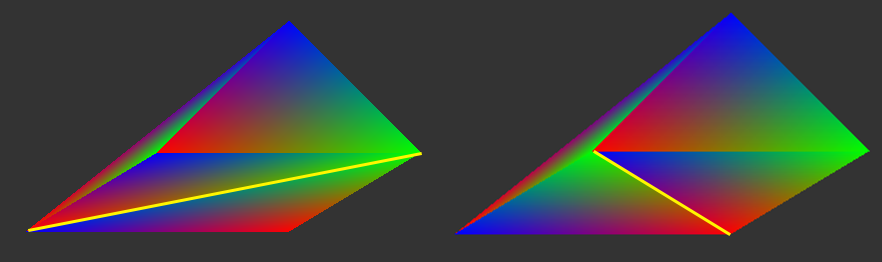
\includegraphics[width=0.8\textwidth]{Captures/BeforeAfterFlip.png}}
	
	\caption{Flip de l'arête jaune dans le triangle de gauche et résultat à droite}
\end{figure}
\FloatBarrier

L'algorithme de Lawson peut aussi être appliqué incrémentalement après chaque insertion de point dans la triangulation plutôt que sur le maillage entier:

\begin{figure}[h!]
	\adjustbox{center}{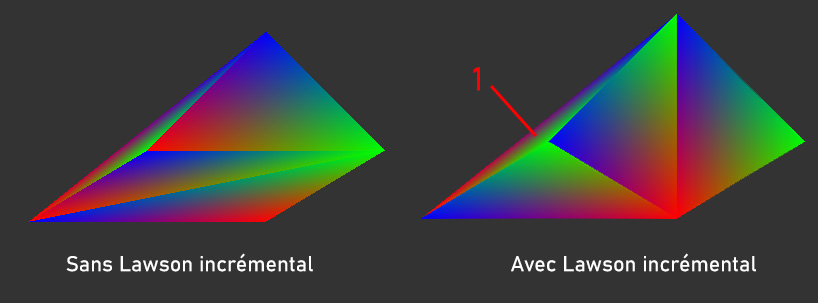
\includegraphics[width=0.8\textwidth]{Captures/InsertOutIncremental.jpg}}
	
	\caption{Insertion de deux points à l'extérieur du triangle de départ comme dans la \figurename \ref{InsertOut} avec et sans l'application de l'algorithme de Lawson incrémental à droite et à gauche respectivement. Le triangle 1 reste très plat à cause de son arête extérieure qui ne peut pas être flippée.}
\end{figure}
\FloatBarrier

\begin{figure}[h!]
	\adjustbox{center}{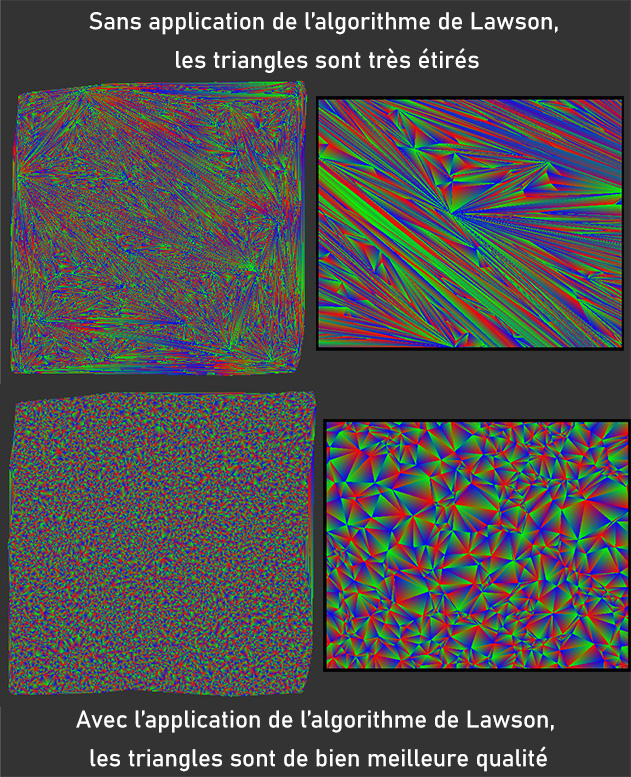
\includegraphics[width=0.8\textwidth]{Captures/TerrainNoVsIncremental.jpg}}
	
	\caption{Comparaison de la qualité des triangles pour l'insertion d'un large nombre de points avec et sans l'application de l'algorithme de Lawson (version incrémentale)}
\end{figure}
\FloatBarrier